\section{Swtich 基本功能描述}


Marvell 88Q5050 是一款具有 8 路端口的交换机芯片,在汽车领域广泛应用。可以配置支持 IEEE 100BASE-T1,100BASE-TX,RGMI/RMII/MII,GMII 和 SGMII 端口。该芯片将低功耗的 Phy 芯片和 MAC 
集成到内部,可满足 IEEE 802.3 标准。IEEE 100BASE-T1 Phy 可满足 OPEN Aliance BroadR-Reach。

\subsection{支持接口}
88Q5050 可支持接口如下:
\begin{itemize}
    \item 4 x IEEE 100BASE-T1 (IEEE 802.3bw)
    \item 额外 6 路可配置端口(同时可打开 4 路)
    \begin{itemize}
        \item 1 x IEEE 100BASE-T1
        \item 1 x IEEE 100BASE-TX
        \item 2 x MII/RMII/RGMII
        \item 1 x MII
        \item 1 x MII
        \item 1 x SGMII 
    \end{itemize}
    \item 2 x SMI
    \item 可配置 GPIO
    \item QSPI 可配置频率 19.2 ~ 83.3 MHz
    \item EEPROM 从接口,可配置E2大小 32 ~ 512 Kb
\end{itemize}

表\ref{tab:port_interface}汇总了芯片接口类型,每一行代表了一种组合。

% Table generated by Excel2LaTeX from sheet 'Sheet1'
\begin{table}[htbp]
    \centering
    
    \caption{Port 接口汇总}
      \begin{tabular}{lllllr}
      \toprule
      Ports 1 to 4 & Port 5 & Port 6 & Port 7 & Port 8 & Notes \\
      \midrule
      100BASE-T1 & 100BASE-T1 & 100BASE-TX & SGMII & xMII  &  \\
      \tabincell{l}{100BASE-T1} & \tabincell{l}{xMII}  & \tabincell{l}{100BASE-TX} & \tabincell{l}{SGMII} & \tabincell{l}{xMII}  & \tabincell{l}{Port 5 6 7是互相关联的,\\任何一个 Port 配置为 MII,RMII,或 RGMII,\\剩余的两个 Port 只可以配置为 PHY 或 SERDES} \\
      100BASE-T1 & 100BASE-T1 & xMII  & SGMII & xMII  &  \\
      100BASE-T1 & 100BASE-T1 & 100BASE-TX & xMII  & xMII  &  \\
      100BASE-T1 & 100BASE-T1 & 100BASE-TX & SGMII & GMII  &  \\
      \bottomrule
      \end{tabular}%
      \label{tab:port_interface}
  \end{table}%
  
\subsection{使用案例}

取决于配置, 88Q5050 可用于不同的应用场合:

\begin{itemize}
    \item 被内部 CPU 管理
    \item 被外部 CPU 管理
    \item 无管理
\end{itemize}

在实际使用中,采用了外部 CPU 驱动和管理 Switch,在这种场景下,Switch 内部的 CPU 被禁止,外部 CPU 可通过 SMI 接口或以太网接口连接和管理 Swtich。
通过 SMI 或以太网接口连接 Swtich 分别如下图所示。

\begin{figure}[ht]
    \centering
    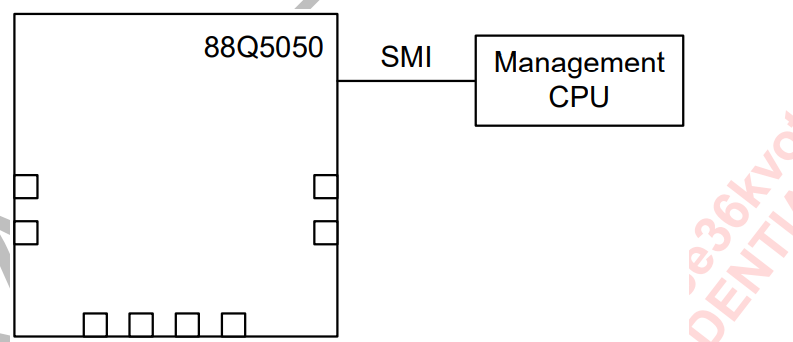
\includegraphics[scale=0.7]{pic/Snipaste_2021-10-23_19-03-03.png}
    \caption{SMI 接口管理 Switch}
    \label{fig:smi_interface}
\end{figure}

\begin{figure}[ht]
    \centering
    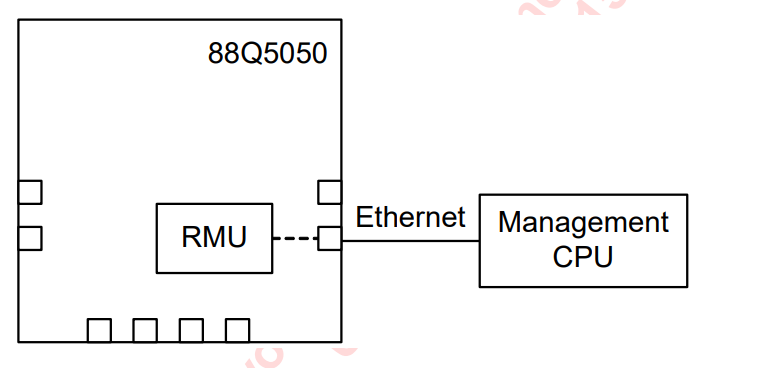
\includegraphics[scale=0.7]{pic/Snipaste_2021-10-23_19-04-54.png}
    \caption{以太网接口管理 Switch}
    \label{fig:eth_interface}
\end{figure}

\section{Swtich 核心}
\subsection{功能描述} 
本节对 Switch 所有端口一致的功能进行描述。Switch 核心的功能分为以下几个部分:

\begin{itemize}
    \item Switch 基础功能:所有帧操作模式通用的功能。
    \item 普通网络帧模式:IEEE 标准下未打 tag 帧和打 tag 帧,或自定义 Swtich 端口且至少有一个 \textbf{Provider} 端口。
    \item \textbf{Provider} 帧模式: IEEE 标准 \textbf{Provider} 端口。
    \item 分布式交换机架构帧模式(Distrubuted Switch Architecture, DSA):多片 Switch 级联或连接到一个 Switch 管理 CPU。
\end{itemize}

每一个 Switch 端口可以在以下几种基础操作模式下:
\begin{itemize}
    \item 普通模式
    \item \textbf{Provider} 模式
    \item DSA 模式,包括经典模式和 \lstinline{EtherType}
\end{itemize}

以上操作模式都通过寄存器 \lstinline{PORT offset 0x04} 的\lstinline{FrameMode} 字段配置。

\subsection{基础 Swtich 功能}
\subsubsection{Swtich 物理数据流向}

88Q5050接收以太网帧,并决定丢弃或从一个或多个端口发送出去。对每个以太网帧执行何种决策只是 Switch 内部任务的一种。
图\ref{fig:data_flow}显示了交换机内部的数据路径以及在帧通过 88q5050 器件时处理帧的主要功能块。每个功能块及其可配置寄存器选项在接下来的章节中描述。
本节主要关注 Switch 内部一个端口上的帧处理及策略。

\begin{figure}[ht]
    \centering
    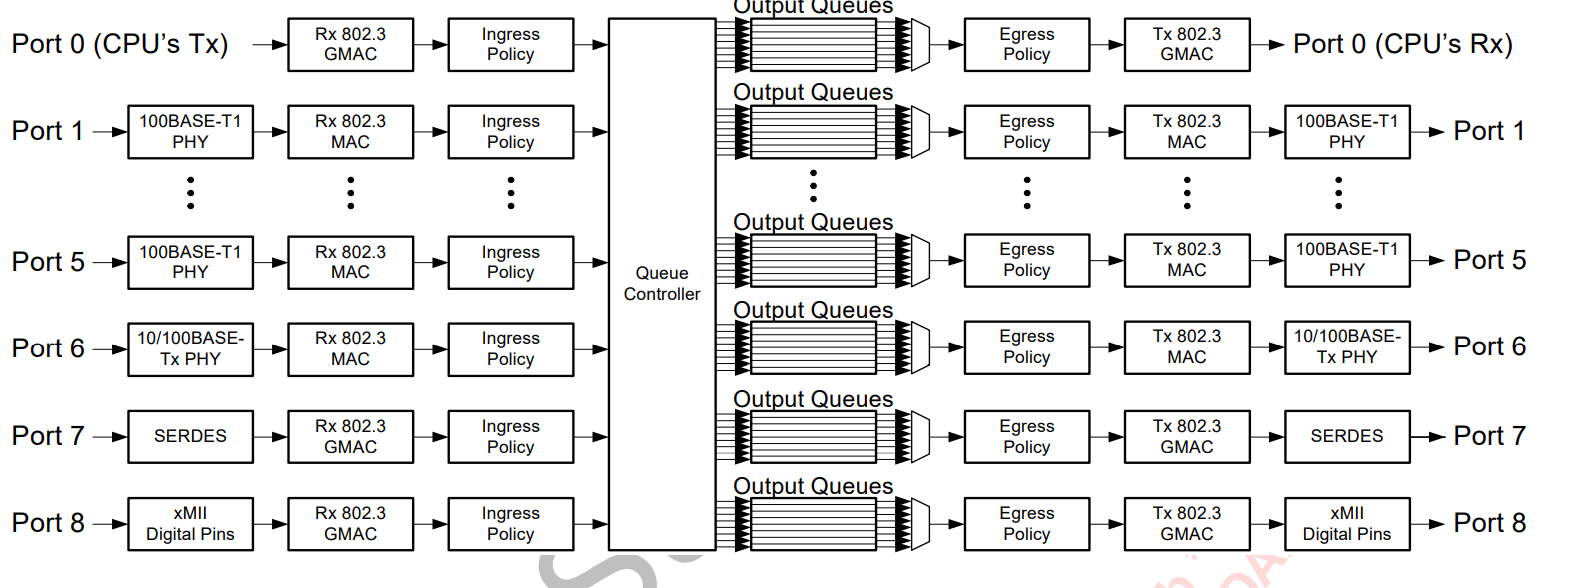
\includegraphics[scale=0.5]{pic/Snipaste_2021-10-24_16-16-48.png}
    \caption{Swtich data flow}
    \label{fig:data_flow}
\end{figure}

\subsubsection{物理接口}
每个端口都包含一个物理接口,用于从端口的 MAC 接收和传输帧。 一些端口支持多种物理接口选项,而一些仅支持部分。如果一个端口支持多个接口选项,则在同一时刻仅能使用一种。
每个端口支持的物理接口选项在\textbf{DataSheet} Device physical interfaces 章节详细描述。

\begin{note}
88q5050 的设备特点通常会和相关寄存器关联。这些寄存器按照分组组织,分别为 \lstinline{PORT},\lstinline{Global1(GLB1)},\lstinline{Global2(GLB2)} 和 \lstinline{TCAM},以及一些访问PHY的寄存器。
每一组包括 32 个 16 位寄存器,每一个端口包括这样的 32 个寄存器。组中超出 32 的特殊寄存器通过 \lstinline{offset} 引用。
如端口控制寄存器通过 \lstinline{PORT offset 0x04} 引用,因为该寄存器位于端口地址空间的 \lstinline{0x04} 地址。详细的寄存器描述可参考 寄存器手册 \textbf{Register specification}。
\end{note}

\subsubsection{介质访问控制(MAC)}
88Q5050 带有 9 个 MAC,执行 802.3 协议的所有功能,包括帧格式,帧裁剪,CRC 校验,载波侦听多路访问/冲突检测增强(CSMA/CD)和碰撞处理。
每一路 MAC 支持 10 和 100M 全双工或半双工模式,及 1G 全双工模式。连接到内部 CPU 的 MAC使用固定的 1G 速率,且只支持全双工模式。

MAC Rx 功能块检查接收到的包,并抛弃存在 CRC 错误、对齐错误和小于 64 字节的短包或大于 1522/2048/10240字节的过长包。
MAC 持续地监测它的接收线,等待前导段字节及其后的帧起始段。接下来的 6 个字节用于包的目的 mac 地址,再接下来的 6 个字节为包的源地址。
这两个地址是 Switch 功能操作的基础。接下来的 2~60个字节被检查,并可用于服务质量(QoS)或交换机做出的策略决定。
最后的 4 个字节是包的帧校验序列(FCS)。FCS 必须满足 IEEE 802.3 CRC32 需求,负责该包会被丢弃。具体格式见图\ref{fig:eth_mac_format}。

\begin{figure}[ht]
    \centering
    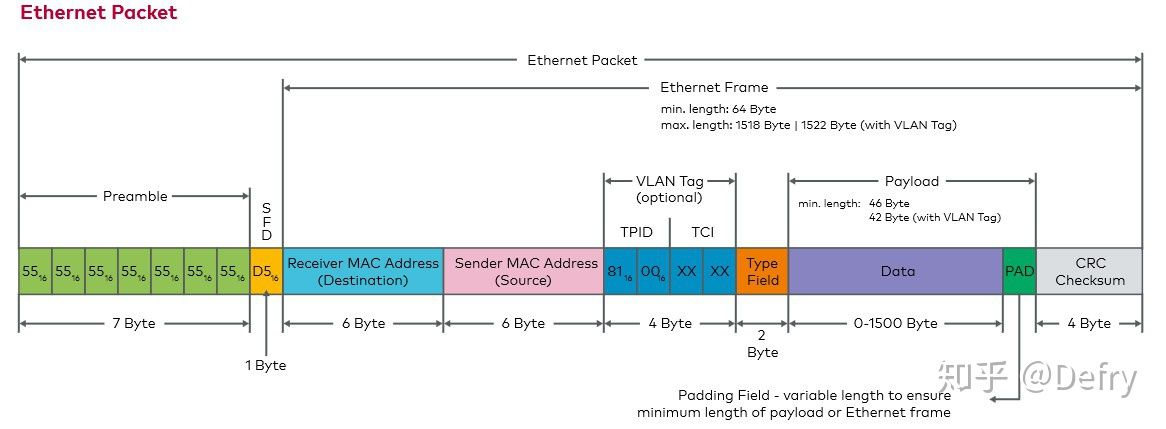
\includegraphics[scale=0.5]{pic/eth_mac_format.jpg}
    \caption{Ethernet mac frame format}
    \label{fig:eth_mac_format}
\end{figure}

在一个包被发送之前,发送功能块会检查发送线是否可用于发送。当端口为全双工模式时,发送线总是处于可用,但是在半双工模式下,可能处于不可发送状态。
一旦发送线时忙碌状态,发送推迟发送,并进行等待。当发送线可用时,发送器确保在发送帧前的 56 位前导码和 8 位 SFD 之前出现至少 96 位的最小包间隙。
实际的帧在 SFD 后立即发送。

在半双工模式下, 88q5050 在发送时监测碰撞信号。如果监测到碰撞(PHY同时在发送和接收数据)。MAC 发送一个拥挤信号(Jam pattern),然后延迟重传一段随机时间,该时间由 IEEE 802.3 
回退算法决定(backoff algorithm)。在全双工模式下则忽略碰撞和回退算法。

\subsubsection{统计计数器}
TODO

\subsubsection{调试计数器}
TODO

\subsection{基础 Switch 操作}

\subsubsection{查表引擎}

\subsubsection{地址搜索或翻译}

\subsubsection{自动地址学习}

\subsubsection{硬件地址学习限制}

\subsubsection{自动地址老化}